\documentclass[10pt]{article}
\usepackage[letterpaper,margin=0.55in]{geometry}
\usepackage[T1]{fontenc}
\usepackage{lmodern}
\usepackage{graphicx}
\usepackage{tabularx}
\usepackage{booktabs}
\usepackage{enumitem}
\usepackage{xcolor}
\usepackage{titlesec}
\usepackage{multicol}

\definecolor{navy}{HTML}{1F3A5F}
\definecolor{soft}{HTML}{EEF2F7}
\titleformat{\section}{\color{navy}\bfseries\normalsize}{}{0pt}{}
\titlespacing*{\section}{0pt}{5pt}{1pt}
\setlist{nosep,leftmargin=1.1em,topsep=1pt}
\setlength{\parindent}{0pt}
\setlength{\parskip}{3pt}
\setlength{\columnsep}{16pt}
\pagestyle{empty}

\begin{document}
\small

{\color{navy}\Large\bfseries Copart, Inc. (NASDAQ: CPRT)}\hfill{\color{navy}\bfseries\Large SHORT}\\[1pt]
{\footnotesize Price \$27.36 (Sep 30, 2026) \quad|\quad Price target \$21.50 ($-$21\%) \quad|\quad Market cap \$25.3B \quad|\quad 17.6x P/E \quad|\quad 11.1x EV/EBITDA \quad|\quad 6--12 mo.}

\vspace{3pt}
\colorbox{soft}{\parbox{\dimexpr\linewidth-2\fboxsep}{
\textbf{Recommendation: short CPRT, price target \$21.50 (21\% downside).} Copart runs a toll road on wrecked cars, and fewer cars are using the road. U.S. collision claim frequency keeps falling ($-$3.4\% y/y). Drivers carry higher deductibles and skip small claims, and cars are getting harder to crash. Inside that shrinking pool, Copart is losing share to its only real rival, IAA. The stock is down 57\% and a 17.6x P/E looks cheap next to a 34x ten-year median, so the bull case is ``buy the dip.'' We think it is a value trap. Earnings are falling for the first time in any of Copart's major drawdowns, and consensus still expects FY27 EPS growth of 11\%. We see FY27 EPS 18\% below the Street.}}

\section{Company overview}
Copart sells wrecked and unwanted vehicles through online auctions in the U.S. and abroad (international was 19\% of Q4 FY26 revenue). When an insurer decides a car costs more to fix than it is worth, it declares a total loss and consigns the car to Copart. Copart tows it, stores it, lists it and sells it to rebuilders, dismantlers, exporters and dealers, and 38\% of U.S. units go to international buyers. Copart keeps buyer and seller fees; the insurer keeps the proceeds. Roughly 80\% of volume comes from insurance companies. FY26 (July year-end) revenue was \$4.67B (85\% service fees), operating income \$1.65B and EPS \$1.55. Copart has \$4.5B of cash and securities, no meaningful debt, and bought back \$1.6B of stock in FY26. In September 2026 it agreed to buy ACV Auctions, a dealer-to-dealer wholesale marketplace, for \$10.50 per share in cash ($\sim$\$1.8B).

\section{Industry: a two-player market fed by insurance claims}
U.S. salvage auctions are effectively a duopoly: Copart and IAA (owned by RB Global since 2023). Supply follows a simple chain: \emph{crash $\rightarrow$ claim $\rightarrow$ total loss $\rightarrow$ auction.} Two forces pull in opposite directions. Rising repair costs (+57\% since 2019) push more claimed cars into total losses, so total-loss frequency hit a record 23.3\% in Q2 2026, up from 15.6\% in 2015. That lifts the price of each car. But the number of claims is falling, and Copart is paid per car. A higher total-loss rate cannot offset a shrinking base of claims forever: total losses are already nearly a quarter of claims.

\section{Thesis 1: The supply of wrecked cars is in structural decline}
\begin{itemize}
  \item \textbf{Fewer claims, not fewer miles.} U.S. collision claim frequency fell 3.4\% y/y in Copart's latest quarter, after $-$7.5\% in the quarter to October 2025. Repairable claims fell 9.7\% in 2025 (CCC). Yet miles driven are up 2.5\% vs.\ 2019. People still crash; they file less.
  \item \textbf{Insurance got expensive, so drivers self-insure.} Auto insurance prices are up 49\% since 2019 and repair prices up 57\%. 26\% of policyholders now carry a \$1,000+ deductible, and 7\% skipped a claim over rate worries (J.D. Power). Insured vehicle-years (earned car years) fell $\sim$4\% y/y. Every dropped collision policy removes a potential Copart car.
  \item \textbf{Cars are getting harder to crash.} Automatic emergency braking cuts rear-end crashes by $\sim$50\% (IIHS), and NHTSA makes it mandatory on all new light vehicles from September 2029. As the fleet turns over, crash frequency keeps falling for a decade. This is structural, not cyclical.
\end{itemize}

\section{Thesis 2: Copart is losing share inside a shrinking market}
\begin{itemize}
  \item \textbf{IAA is taking share every quarter.} Over the same 12 months, IAA's automotive lots grew 5.4\% while Copart's units fell 5.5\%. The combined pool fell only 1.6\%, so most of Copart's decline is lost share. Its share of the two-player pool fell \textbf{from 63.9\% to 61.4\%}: about \textbf{167k units and \$166M of service revenue} a year (Exhibit 1B).
  \item \textbf{The fastest-growing insurer favors the rival.} Management said Q4 FY26 U.S. insurance assignments would have \emph{grown} 2.3\% without one lost customer, vs.\ a 7.5\% decline reported. That customer was $\sim$10\% of Copart's U.S. insurance volume. Industry reports identify it as Progressive, which became the largest U.S. auto insurer in 2026 and now sends $\sim$90\% of its salvage to IAA. Share is following the insurer that is winning share.
  \item \textbf{IAA fixed its weakness.} Under RB Global, IAA cut cycle times by nearly a week and has beaten the market on units for six straight quarters. Copart's historic edge over a poorly run rival is narrowing.
\end{itemize}

\section{Thesis 3: Falling earnings make the ``cheap'' multiple a trap}
\begin{itemize}
  \item \textbf{Margins are already breaking.} In Q4 FY26 revenue rose 2.4\%, but gross profit fell 5.5\%, operating income fell 10.6\% and EPS fell 14.6\%. Yards have fixed costs, and U.S. facility cost per unit rose 14.2\% as volume fell. Higher prices per car (+5.4\% revenue per unit) are no longer enough.
  \item \textbf{A tenth of EPS is interest income, and it is shrinking.} FY26 other income, mostly Treasury bill interest, was \$182M, about 10\% of net income. The ACV deal spends $\sim$\$1.8B of that cash, costing $\sim$\$0.06 of EPS before ACV's own losses. Management guides ACV to breakeven, not accretion, until FY28.
  \item \textbf{This drawdown is different.} In each of Copart's five prior 30\%+ drawdowns with earnings data, trailing EPS was still growing 10--46\%, so buying the dip worked. Today trailing EPS is down 3\% and falling. After weekly oversold signals since 1996, the stock's median 6-month return was $-$0.3\%, vs.\ +9.9\% on a random day.
\end{itemize}

\vspace{2pt}
{\centering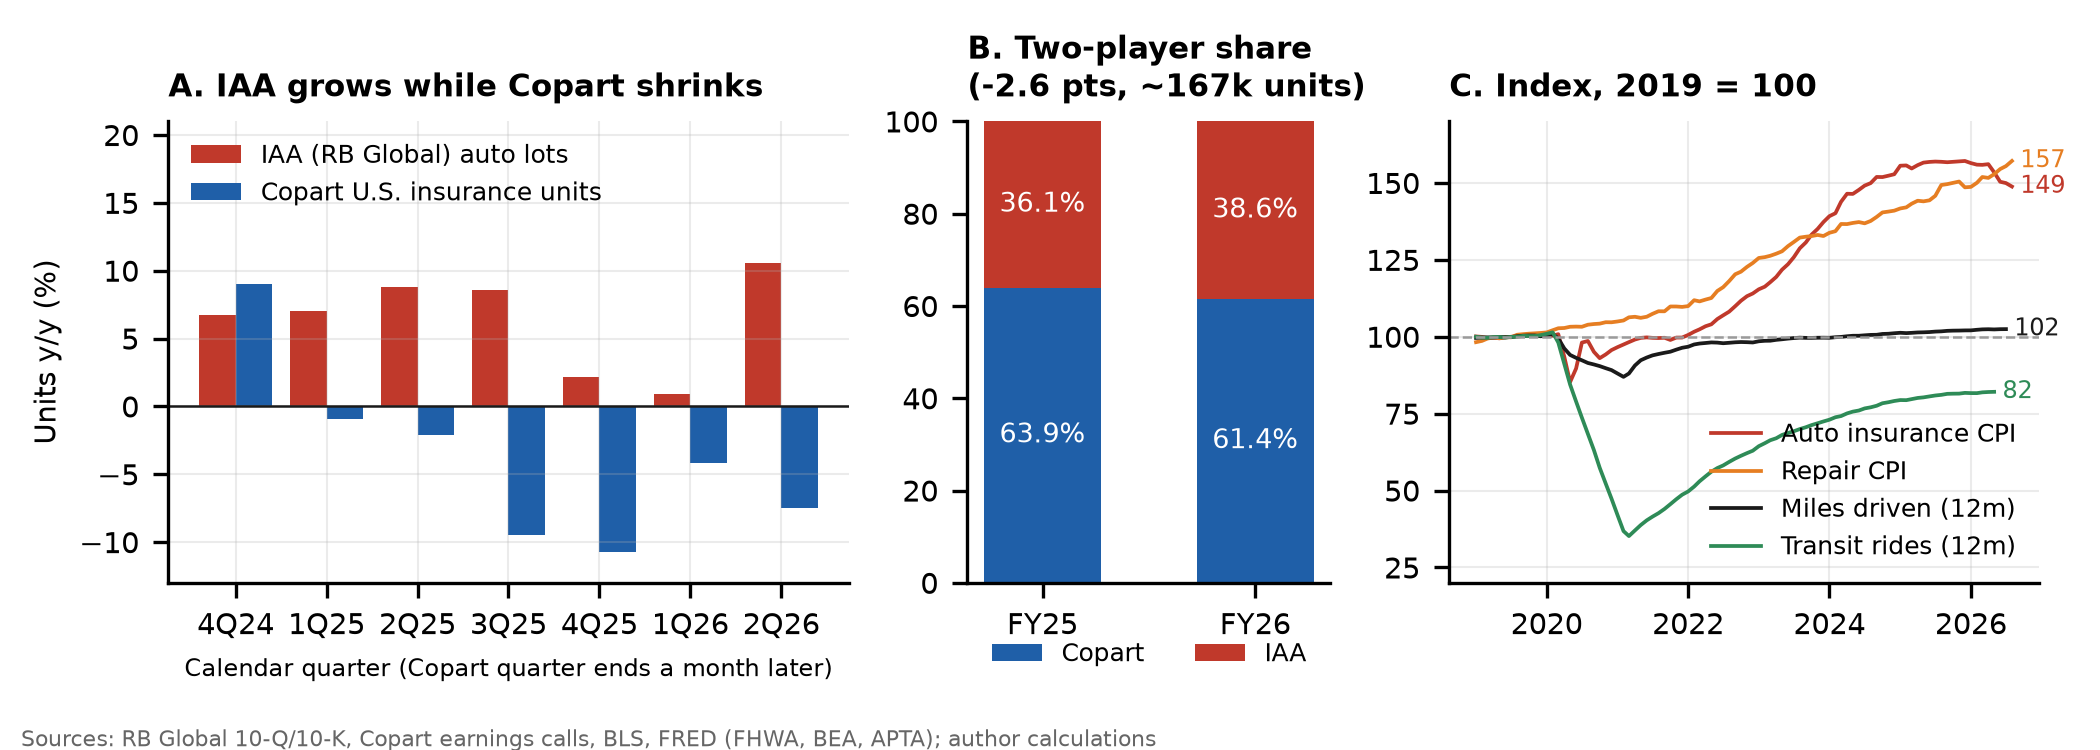
\includegraphics[width=0.92\linewidth]{../model/fundamentals/output/industry_figure.png}\par}
{\centering\footnotesize\textbf{Exhibit 1.} Unit growth, IAA vs.\ Copart U.S. insurance (A); share of the Copart + IAA salvage pool (B); insurance and repair prices, miles driven and transit ridership, 2019 = 100 (C).\par}

\section{Valuation: FY27 EPS of \$1.44, 18\% below consensus}
We build FY27 EPS from units, revenue per unit and margin. In the base case, units fall 3\% as the lost insurer and falling claims carry into the first half, and revenue per unit rises 4\% on higher car values. Operating margin settles at 33\%, near the Q4 FY26 exit rate of 32\%, and other income falls to \$110M after the ACV payment. That gives \textbf{EPS of \$1.44 vs.\ the Street's \$1.75}. At 15x, a discount to share-gaining RB Global (16.8x forward) and a premium to salvage-parts buyer LKQ (7.4x), the base target is \textbf{\$21.50}. That implies 9.7x EV/EBITDA, below today's 11.1x.

\begin{center}
{\footnotesize
\begin{tabular}{@{}lrrrrrrrr@{}}
\toprule
Scenario (prob.) & Units & Rev./unit & Op. margin & FY27 EPS & vs.\ Street & P/E & Target & vs.\ price \\
\midrule
Bear (25\%) & $-$6\% & +3\% & 31.0\% & \$1.30 & $-$26\% & 13x & \$16.84 & $-$38\% \\
\textbf{Base (50\%)} & $\mathbf{-3\%}$ & \textbf{+4\%} & \textbf{33.0\%} & \textbf{\$1.44} & $\mathbf{-18\%}$ & \textbf{15x} & \textbf{\$21.54} & $\mathbf{-21\%}$ \\
Bull (25\%) & +2\% & +5\% & 36.5\% & \$1.70 & $-$3\% & 20x & \$33.90 & +24\% \\
\midrule
\multicolumn{7}{@{}l}{Probability-weighted} & \$23.45 & $-$14\% \\
\bottomrule
\end{tabular}}
\end{center}
\vspace{-4pt}
Probability-weighted, the expected downside ($\sim$20 pts) is more than 3x the expected upside ($\sim$6 pts), and even the bull case needs a unit recovery that no data point supports today.

\section{Catalysts}
\begin{itemize}
  \item \textbf{Q1 FY27 earnings (Nov 19, 2026).} Consensus is \$0.40 vs.\ \$0.41 a year ago. Another quarter of falling U.S. insurance units and cost-per-unit growth should push FY27 estimates toward our \$1.44.
  \item \textbf{RB Global Q3 results (early Nov 2026).} A seventh straight quarter of IAA unit gains would confirm the share shift is not a one-customer event.
  \item \textbf{ACV closing (by end of 2026).} Cash leaves the balance sheet, interest income falls, and ACV's losses consolidate. That exposes Copart to dealer wholesale, a market led by Manheim and OPENLANE where Copart has no edge.
  \item \textbf{Monthly claims data.} Continued declines in collision frequency and repairable claims (CCC, insurer disclosures) keep pressure on the unit outlook.
\end{itemize}

\section{Risks and mitigants}
{\footnotesize
\begin{tabularx}{\linewidth}{@{}p{0.29\linewidth}X@{}}
\toprule
Risk & Mitigant \\
\midrule
Claims recover as insurance prices fall (auto insurance CPI $-$5.1\% y/y) & Repair prices are still rising (+7.8\% y/y) and deductibles are sticky, so small claims stay unfiled. AEB lowers crash frequency whatever insurance costs. We cover if collision frequency turns positive for two quarters. \\
Easier comps once the lost customer laps in early 2027 & The base case already assumes a smaller decline (units $-$3\%). The margin and interest-income pressure does not depend on the comp. \\
Hurricane season brings a burst of catastrophe volume & Catastrophe units are one-off and flatter revenue and units, not the trend. Copart reports volumes ex-catastrophe. \\
Buybacks and the ACV story support the stock & ACV uses $\sim$\$1.8B of the cash that funded buybacks. Short interest is only 4.6\% of float (3.3 days to cover), so squeeze risk is low. \\
Stock already down 57\% & Cheap on trailing P/E, but on our FY27 EPS the stock trades at 19x with falling units. We size the position with a stop at \$32.60 (above the 50-day average and the 23.6\% retracement). \\
\bottomrule
\end{tabularx}}

\vspace{2pt}
{\scriptsize\color{gray} Sources: Copart FY2026 10-K and Q4 FY26 earnings release and calls (FY25--FY26); RB Global 10-Q/10-K filings; CCC Intelligent Solutions Crash Course 2026; J.D. Power 2025 U.S. Auto Claims Satisfaction Study; IIHS; NHTSA FMVSS 127; BLS CPI; FRED (FHWA, APTA); Yahoo Finance prices and consensus (Sep 30, 2026); industry press on insurer allocations. Share estimates use Copart's stated $>$4M FY26 units; the share shift is $-$2.5 to $-$2.6 pts across a 4.0--4.5M unit range. Estimates and targets are the authors'.\par}
\end{document}
